\chapter{Project: Skill-Sharing Website}\label{skillsharing}

\epigraphhead[30]{
\epigraph{\hspace*{-.1cm}\itshape``If you have knowledge, let others light their candles at it.''}%
{---Margaret Fuller}
}\index{skill-sharing project}\index{meetup}\index{project chapter}

A \emph{\index{skill-sharing}skill-sharing} meeting is an event where people with a shared interest come together and give small, informal presentations about things they know. At a \index{gardening}gardening skill-sharing meeting, someone might explain how to cultivate \index{celery}celery. Or in a programming skill-sharing group, you could drop by and tell people about Node.js.\index{learning}\index{users' group}

Such meetups—also often called \emph{users' groups} when they are about computers—are a great way to broaden your horizon, learn about new developments, or simply meet people with similar interests. Many larger cities have JavaScript meetups. They are typically free to attend, and I've found the ones I've visited to be friendly and welcoming.

In this final project chapter, our goal is to set up a \index{website}website for managing \index{talk}talks given at a skill-sharing meeting. Imagine a small group of people meeting up regularly in the office of one of the members to talk about \index{unicycling}unicycling. The previous organizer of the meetings moved to another town, and nobody stepped forward to take over this task. We want a system that will let the participants propose and discuss talks among themselves, without a central organizer.

 The full code for the project can be \index{download}downloaded from \href{https://eloquentjavascript.net/code/skillsharing.zip}{\emph{https://eloquentjavascript.net\slash code\slash skillsharing.zip}}.

\section{Design}\index{skill-sharing project}\index{persistence}

There is a \emph{\index{server}server} part to this project, written for \index{Node.js}Node.js, and a \emph{\index{client}client} part, written for the \index{browser}browser. The server stores the system's data and provides it to the client. It also serves the files that implement the client-side system.\index{HTTP!client}

The server keeps the list of \index{talk}talks proposed for the next meeting, and the client shows this list. Each talk has a presenter name, a title, a summary, and an array of \index{comment}comments associated with it. The client allows users to propose new talks (adding them to the list), delete talks, and comment on existing talks. Whenever the user makes such a change, the client makes an HTTP \index{request}request to tell the server about it.

\vskip 1.5ex
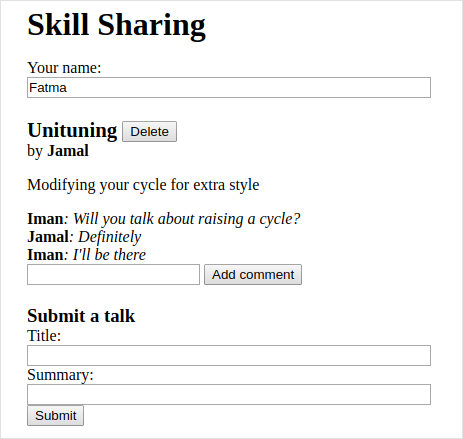
\includegraphics[width=10cm]{img/skillsharing.png}
\vskip 1.5ex\index{live view}\index{user experience}\index{pushing data}\index{connection}

The \index{application}application will be set up to show a \emph{live} view of the current proposed talks and their comments. Whenever someone, somewhere, submits a new talk or adds a comment, all people who have the page open in their browsers should immediately see the change. This poses a bit of a challenge—there is no way for a web server to open a connection to a client, nor is there a good way to know which clients are currently looking at a given website.\index{Node.js}

A common solution to this problem is called \emph{\index{long polling}long polling}, which happens to be one of the motivations for Node's design.

\section{Long polling}\index{firewall}\index{notification}\index{long polling}\index{network}\index{browser!security}

To be able to immediately notify a client that something changed, we need a \index{connection}connection to that client. Since web browsers do not traditionally accept connections and clients are often behind \index{router}routers that would block such connections anyway, having the server initiate this connection is not practical.

We can arrange for the client to open the connection and keep it around so that the server can use it to send information when it needs to do so.\index{socket}

But an \index{HTTP}HTTP request allows only a simple flow of information: the client sends a request, the server comes back with a single response, and that is it. There is a technology called \emph{\index{WebSockets}WebSockets}, supported by modern browsers, that makes it possible to open \index{connection}connections for arbitrary data exchange. But using them properly is somewhat tricky.

In this chapter, we use a simpler technique—\index{long polling}long polling—where clients continuously ask the server for new information using regular HTTP requests, and the server stalls its answer when it has nothing new to report.\index{live view}

As long as the client makes sure it constantly has a polling request open, it will receive information from the server quickly after it becomes available. For example, if Fatma has our skill-sharing application open in her browser, that browser will have made a request for updates and will be waiting for a response to that request. When Iman submits a talk on Extreme Downhill Unicycling, the server will notice that Fatma is waiting for updates and send a response containing the new talk to her pending request. Fatma's browser will receive the data and update the screen to show the talk.\index{robustness}\index{timeout}

To prevent connections from timing out (being aborted because of a lack of activity), \index{long polling}long polling techniques usually set a maximum time for each request, after which the server will respond anyway, even though it has nothing to report, after which the client will start a new request. Periodically restarting the request also makes the technique more robust, allowing clients to recover from temporary \index{connection}connection failures or server problems.\index{Node.js}

A busy server that is using long polling may have thousands of waiting requests, and thus \index{TCP}TCP connections, open. Node, which makes it easy to manage many connections without creating a separate thread of control for each one, is a good fit for such a system.

\section{HTTP interface}\index{skill-sharing project}\index{interface!HTTP}

Before we start designing either the server or the client, let's think about the point where they touch: the \index{HTTP}HTTP interface over which they communicate.\index{path!URL}\index{method!HTTP}

We will use \index{JSON}JSON as the format of our request and response body. Like in the file server from \hyperref[node.file_server]{Chapter 20}, we'll try to make good use of HTTP methods and \index{header}headers. The interface is centered around the \lstinline`/talks` path. Paths that do not start with \lstinline`/talks` will be used for serving \index{static file}static files—the HTML and JavaScript code for the client-side system.\index{GET method}

A \lstinline`GET` request to \lstinline`/talks` returns a JSON document like this:

\begin{lstlisting}
[{"title": "Unituning",
  "presenter": "Jamal",
  "summary": "Modifying your cycle for extra style",
  "comments": []}]}
\end{lstlisting}
\noindent\index{PUT method}\index{URL}

Creating a new talk is done by making a \lstinline`PUT` request to a URL like \lstinline`/talks/Unituning`, where the part after the second slash is the title of the talk. The \lstinline`PUT` request's body should contain a \index{JSON}JSON object that has \lstinline`presenter` and \lstinline`summary` properties.\index{encodeURIComponent function}\index{escaping!in URLs}\index{whitespace!in URLs}

Since talk titles may contain spaces and other characters that may not appear normally in a URL, title strings must be encoded with the \lstinline`encodeURIComponent` function when building up such a URL.

\begin{lstlisting}
console.log("/talks/" + encodeURIComponent("How to Idle"));
// → /talks/How%20to%20Idle
\end{lstlisting}
\noindent

A request to create a talk about idling might look something like this:

\begin{lstlisting}
PUT /talks/How%20to%20Idle HTTP/1.1
Content-Type: application/json
Content-Length: 92

{"presenter": "Maureen",
 "summary": "Standing still on a unicycle"}
\end{lstlisting}
\noindent

Such URLs also support \lstinline`GET` requests to retrieve the JSON representation of a talk and \lstinline`DELETE` requests to delete a talk.\index{POST method}

Adding a \index{comment}comment to a talk is done with a \lstinline`POST` request to a URL like \lstinline`/talks/Unituning/comments`, with a JSON body that has \lstinline`author` and \lstinline`message` properties.

\begin{lstlisting}
POST /talks/Unituning/comments HTTP/1.1
Content-Type: application/json
Content-Length: 72

{"author": "Iman",
 "message": "Will you talk about raising a cycle?"}
\end{lstlisting}
\noindent\index{query string}\index{timeout}\index{ETag header}\index{If-None-Match header}

To support \index{long polling}long polling, \lstinline`GET` requests to \lstinline`/talks` may include extra headers that inform the server to delay the response if no new information is available. We'll use a pair of headers normally intended to manage caching: \lstinline`ETag` and \lstinline`If-None-Match`.\index{304 (HTTP status code)}

Servers may include an \lstinline`ETag` (``entity tag'') header in a response. Its value is a string that identifies the current version of the resource. Clients, when they later request that resource again, may make a \emph{\index{conditional request}conditional request} by including an \lstinline`If-None-Match` header whose value holds that same string. If the resource hasn't changed, the server will respond with status code 304, which means ``not modified'', telling the client that its cached version is still current. When the tag does not match, the server responds as normal.\index{Prefer header}

We need something like this, where the client can tell the server which version of the list of talks it has, and the server responds only when that list has changed. But instead of immediately returning a 304 response, the server should stall the response and return only when something new is available or a given amount of time has elapsed. To distinguish long polling requests from normal conditional requests, we give them another header, \lstinline`Prefer: wait=90`, which tells the server that the client is willing to wait up to 90 seconds for the response.

The server will keep a version number that it updates every time the talks change and will use that as the \lstinline`ETag` value. Clients can make requests like this to be notified when the talks change:

\begin{lstlisting}
GET /talks HTTP/1.1
If-None-Match: "4"
Prefer: wait=90

(time passes)

HTTP/1.1 200 OK
Content-Type: application/json
ETag: "5"
Content-Length: 295

[....]
\end{lstlisting}
\noindent\index{security}

The protocol described here does not do any \index{access control}access control. Everybody can comment, modify talks, and even delete them. (Since the Internet is full of \index{hooligan}hooligans, putting such a system online without further protection probably wouldn't end well.)

\section{The server}\index{skill-sharing project}

Let's start by building the \index{server}server-side part of the program. The code in this section runs on \index{Node.js}Node.js.

\subsection{Routing}\index{createServer function}\index{path!URL}\index{method!HTTP}

Our server will use \lstinline`createServer` to start an HTTP server. In the function that handles a new request, we must distinguish between the various kinds of requests (as determined by the method and the path) that we support. This can be done with a long chain of \lstinline`if` statements, but there is a nicer way.\index{dispatch}

A \emph{\index{router}router} is a component that helps dispatch a request to the function that can handle it. You can tell the router, for example, that \lstinline`PUT` requests with a path that matches the regular expression \lstinline`/^\/talks\/([^\/]+)$/` (\lstinline`/talks/` followed by a talk title) can be handled by a given function. In addition, it can help extract the meaningful parts of the path (in this case the talk title), wrapped in parentheses in the \index{regular expression}regular expression, and pass them to the handler function.

There are a number of good router packages on \index{NPM}NPM, but here we'll write one ourselves to illustrate the principle.\index{require function}\index{Router class}\index{module}

This is \lstinline`router.js`, which we will later \lstinline`require` from our server module:

\begin{lstlisting}
const {parse} = require("url");

module.exports = class Router {
  constructor() {
    this.routes = [];
  }
  add(method, url, handler) {
    this.routes.push({method, url, handler});
  }
  resolve(context, request) {
    let path = parse(request.url).pathname;

    for (let {method, url, handler} of this.routes) {
      let match = url.exec(path);
      if (!match || request.method != method) continue;
      let urlParts = match.slice(1).map(decodeURIComponent);
      return handler(context, ...urlParts, request);
    }
    return null;
  }
};
\end{lstlisting}
\noindent\index{Router class}

The module exports the \lstinline`Router` class. A router object allows new handlers to be registered with the \lstinline`add` method and can resolve requests with its \lstinline`resolve` method.\index{some method}

The latter will return a response when a handler was found, and \lstinline`null` otherwise. It tries the routes one at a time (in the order in which they were defined) until a matching one is found.\index{capture group}\index{decodeURIComponent function}\index{escaping!in URLs}

The handler functions are called with the \lstinline`context` value (which will be the server instance in our case), match strings for any groups they defined in their \index{regular expression}regular expression, and the request object. The strings have to be URL-decoded since the raw URL may contain \lstinline`%20`-style codes.

\subsection{Serving files}

When a request matches none of the request types defined in our router, the server must interpret it as a request for a file in the \lstinline`public` directory. It would be possible to use the file server defined in \hyperref[node.file_server]{Chapter 20} to serve such files, but we neither need nor want to support \lstinline`PUT` and \lstinline`DELETE` requests on files, and we would like to have advanced features such as support for caching. So let's use a solid, well-tested \index{static file}static file server from \index{NPM}NPM instead.\index{createServer function}\index{ecstatic package}

I opted for \lstinline`ecstatic`. This isn't the only such server on NPM, but it works well and fits our purposes. The \lstinline`ecstatic` package exports a function that can be called with a configuration object to produce a request handler function. We use the \lstinline`root` option to tell the server where it should look for files. The handler function accepts \lstinline`request` and \lstinline`response` parameters and can be passed directly to \lstinline`createServer` to create a server that serves \emph{only} files. We want to first check for requests that we should handle specially, though, so we wrap it in another function.

\begin{lstlisting}
const {createServer} = require("http");
const Router = require("./router");
const ecstatic = require("ecstatic");

const router = new Router();
const defaultHeaders = {"Content-Type": "text/plain"};

class SkillShareServer {
  constructor(talks) {
    this.talks = talks;
    this.version = 0;
    this.waiting = [];

    let fileServer = ecstatic({root: "./public"});
    this.server = createServer((request, response) => {
      let resolved = router.resolve(this, request);
      if (resolved) {
        resolved.catch(error => {
          if (error.status != null) return error;
          return {body: String(error), status: 500};
        }).then(({body,
                  status = 200,
                  headers = defaultHeaders}) => {
          response.writeHead(status, headers);
          response.end(body);
        });
      } else {
        fileServer(request, response);
      }
    });
  }
  start(port) {
    this.server.listen(port);
  }
  stop() {
    this.server.close();
  }
}
\end{lstlisting}
\noindent

This uses a similar convention as the file server from the \hyperref[node]{previous chapter} for responses—handlers return promises that resolve to objects describing the response. It wraps the server in an object that also holds its state.

\subsection{Talks as resources}

The \index{talk}talks that have been proposed are stored in the \lstinline`talks` property of the server, an object whose property names are the talk titles. These will be exposed as HTTP \index{resource}resources under \lstinline`/talks/[title]`, so we need to add handlers to our router that implement the various methods that clients can use to work with them.\index{GET method}\index{404 (HTTP status code)}

The handler for requests that \lstinline`GET` a single talk must look up the talk and respond either with the talk's JSON data or with a 404 error response.

\begin{lstlisting}
const talkPath = /^\/talks\/([^\/]+)$/;

router.add("GET", talkPath, async (server, title) => {
  if (title in server.talks) {
    return {body: JSON.stringify(server.talks[title]),
            headers: {"Content-Type": "application/json"}};
  } else {
    return {status: 404, body: `No talk '${title}' found`};
  }
});
\end{lstlisting}
\noindent\index{DELETE method}

Deleting a talk is done by removing it from the \lstinline`talks` object.

\begin{lstlisting}
router.add("DELETE", talkPath, async (server, title) => {
  if (title in server.talks) {
    delete server.talks[title];
    server.updated();
  }
  return {status: 204};
});
\end{lstlisting}
\noindent\index{long polling}\index{updated method}

The \lstinline`updated` method, which we will define \hyperref[skillsharing.updated]{later}, notifies waiting long polling requests about the change.\index{readStream function}\index{body (HTTP)}\index{stream}

To retrieve the content of a request body, we define a function called \lstinline`readStream`, which reads all content from a \index{readable stream}readable stream and returns a promise that resolves to a string.

\begin{lstlisting}
function readStream(stream) {
  return new Promise((resolve, reject) => {
    let data = "";
    stream.on("error", reject);
    stream.on("data", chunk => data += chunk.toString());
    stream.on("end", () => resolve(data));
  });
}
\end{lstlisting}
\noindent\index{validation}\index{input}\index{PUT method}

One handler that needs to read request bodies is the \lstinline`PUT` handler, which is used to create new \index{talk}talks. It has to check whether the data it was given has \lstinline`presenter` and \lstinline`summary` properties, which are strings. Any data coming from outside the system might be nonsense, and we don't want to corrupt our internal data model or \index{crash}crash when bad requests come in.\index{updated method}

If the data looks valid, the handler stores an object that represents the new talk in the \lstinline`talks` object, possibly \index{overwriting}overwriting an existing talk with this title, and again calls \lstinline`updated`.

\begin{lstlisting}
router.add("PUT", talkPath,
           async (server, title, request) => {
  let requestBody = await readStream(request);
  let talk;
  try { talk = JSON.parse(requestBody); }
  catch (_) { return {status: 400, body: "Invalid JSON"}; }

  if (!talk ||
      typeof talk.presenter != "string" ||
      typeof talk.summary != "string") {
    return {status: 400, body: "Bad talk data"};
  }
  server.talks[title] = {title,
                         presenter: talk.presenter,
                         summary: talk.summary,
                         comments: []};
  server.updated();
  return {status: 204};
});
\end{lstlisting}
\noindent\index{validation}\index{readStream function}

Adding a \index{comment}comment to a \index{talk}talk works similarly. We use \lstinline`readStream` to get the content of the request, validate the resulting data, and store it as a comment when it looks valid.

\begin{lstlisting}
router.add("POST", /^\/talks\/([^\/]+)\/comments$/,
           async (server, title, request) => {
  let requestBody = await readStream(request);
  let comment;
  try { comment = JSON.parse(requestBody); }
  catch (_) { return {status: 400, body: "Invalid JSON"}; }

  if (!comment ||
      typeof comment.author != "string" ||
      typeof comment.message != "string") {
    return {status: 400, body: "Bad comment data"};
  } else if (title in server.talks) {
    server.talks[title].comments.push(comment);
    server.updated();
    return {status: 204};
  } else {
    return {status: 404, body: `No talk '${title}' found`};
  }
});
\end{lstlisting}
\noindent\index{404 (HTTP status code)}

Trying to add a comment to a nonexistent talk returns a 404 error.

\subsection{Long polling support}

The most interesting aspect of the server is the part that handles \index{long polling}long polling. When a \lstinline`GET` request comes in for \lstinline`/talks`, it may be either a regular request or a long polling request.\index{talkResponse method}\index{ETag header}

There will be multiple places in which we have to send an array of talks to the client, so we first define a helper method that builds up such an array and includes an \lstinline`ETag` header in the response.

\begin{lstlisting}
SkillShareServer.prototype.talkResponse = function() {
  let talks = [];
  for (let title of Object.keys(this.talks)) {
    talks.push(this.talks[title]);
  }
  return {
    body: JSON.stringify(talks),
    headers: {"Content-Type": "application/json",
              "ETag": `"${this.version}"`}
  };
};
\end{lstlisting}
\noindent\index{query string}\index{url package}\index{parsing}

The handler itself needs to look at the request headers to see whether \lstinline`If-None-Match` and \lstinline`Prefer` headers are present. Node stores headers, whose names are specified to be case insensitive, under their lowercase names.

\begin{lstlisting}
router.add("GET", /^\/talks$/, async (server, request) => {
  let tag = /"(.*)"/.exec(request.headers["if-none-match"]);
  let wait = /\bwait=(\d+)/.exec(request.headers["prefer"]);
  if (!tag || tag[1] != server.version) {
    return server.talkResponse();
  } else if (!wait) {
    return {status: 304};
  } else {
    return server.waitForChanges(Number(wait[1]));
  }
});
\end{lstlisting}
\noindent\index{long polling}\index{waitForChanges method}\index{If-None-Match header}\index{Prefer header}

If no tag was given or a tag was given that doesn't match the server's current version, the handler responds with the list of talks. If the request is conditional and the talks did not change, we consult the \lstinline`Prefer` header to see whether we should delay the response or respond right away.\index{304 (HTTP status code)}\index{setTimeout function}\index{timeout}\index{callback function}

Callback functions for delayed requests are stored in the server's \lstinline`waiting` array so that they can be notified when something happens. The \lstinline`waitForChanges` method also immediately sets a timer to respond with a 304 status when the request has waited long enough.

\begin{lstlisting}
SkillShareServer.prototype.waitForChanges = function(time) {
  return new Promise(resolve => {
    this.waiting.push(resolve);
    setTimeout(() => {
      if (!this.waiting.includes(resolve)) return;
      this.waiting = this.waiting.filter(r => r != resolve);
      resolve({status: 304});
    }, time * 1000);
  });
};
\end{lstlisting}
\noindent\index{updated method}

\label{skillsharing.updated}Registering a change with \lstinline`updated` increases the \lstinline`version` property and wakes up all waiting requests.

\begin{lstlisting}
SkillShareServer.prototype.updated = function() {
  this.version++;
  let response = this.talkResponse();
  this.waiting.forEach(resolve => resolve(response));
  this.waiting = [];
};
\end{lstlisting}
\noindent\index{HTTP!server}

That concludes the server code. If we create an instance of \lstinline`SkillShareServer` and start it on port 8000, the resulting HTTP server serves files from the \lstinline`public` subdirectory alongside a talk-managing interface under the \lstinline`/talks` URL.

\begin{lstlisting}
new SkillShareServer(Object.create(null)).start(8000);
\end{lstlisting}
\noindent

\section{The client}\index{skill-sharing project}

The \index{client}client-side part of the skill-sharing website consists of three files: a tiny HTML page, a style sheet, and a JavaScript file.

\subsection{HTML}\index{index.html}

It is a widely used convention for web servers to try to serve a file named \lstinline`index.html` when a request is made directly to a path that corresponds to a directory. The \index{file server}file server module we use, \lstinline`ecstatic`, supports this convention. When a request is made to the path \lstinline`/`, the server looks for the file \lstinline`./public/index.html` (\lstinline`./public` being the root we gave it) and returns that file if found.

Thus, if we want a page to show up when a browser is pointed at our server, we should put it in \lstinline`public/index.html`. This is our index file:

\begin{lstlisting}
<!doctype html>
<meta charset="utf-8">
<title>Skill Sharing</title>
<link rel="stylesheet" href="skillsharing.css">

<h1>Skill Sharing</h1>

<script src="skillsharing_client.js"></script>
\end{lstlisting}
\noindent\index{CSS}

It defines the document \index{title}title and includes a style sheet, which defines a few styles to, among other things, make sure there is some space between talks.

At the bottom, it adds a heading at the top of the page and loads the script that contains the \index{client}client-side application.

\subsection{Actions}

The application state consists of the list of talks and the name of the user, and we'll store it in a \lstinline`{talks, user}` object. We don't allow the user interface to directly manipulate the state or send off HTTP requests. Rather, it may emit \emph{actions} that describe what the user is trying to do.\index{handleAction function}

The \lstinline`handleAction` function takes such an action and makes it happen. Because our state updates are so simple, state changes are handled in the same function.

\begin{lstlisting}
function handleAction(state, action) {
  if (action.type == "setUser") {
    localStorage.setItem("userName", action.user);
    return Object.assign({}, state, {user: action.user});
  } else if (action.type == "setTalks") {
    return Object.assign({}, state, {talks: action.talks});
  } else if (action.type == "newTalk") {
    fetchOK(talkURL(action.title), {
      method: "PUT",
      headers: {"Content-Type": "application/json"},
      body: JSON.stringify({
        presenter: state.user,
        summary: action.summary
      })
    }).catch(reportError);
  } else if (action.type == "deleteTalk") {
    fetchOK(talkURL(action.talk), {method: "DELETE"})
      .catch(reportError);
  } else if (action.type == "newComment") {
    fetchOK(talkURL(action.talk) + "/comments", {
      method: "POST",
      headers: {"Content-Type": "application/json"},
      body: JSON.stringify({
        author: state.user,
        message: action.message
      })
    }).catch(reportError);
  }
  return state;
}
\end{lstlisting}
\noindent\index{localStorage object}

We'll store the user's name in \lstinline`localStorage` so that it can be restored when the page is loaded.\index{fetch function}\index{status property}

The actions that need to involve the server make network requests, using \lstinline`fetch`, to the HTTP interface described earlier. We use a wrapper function, \lstinline`fetchOK`, which makes sure the returned promise is rejected when the server returns an error code.

\begin{lstlisting}
function fetchOK(url, options) {
  return fetch(url, options).then(response => {
    if (response.status < 400) return response;
    else throw new Error(response.statusText);
  });
}
\end{lstlisting}
\noindent\index{talkURL function}\index{encodeURIComponent function}

This helper function is used to build up a \index{URL}URL for a talk with a given title.

\begin{lstlisting}
function talkURL(title) {
  return "talks/" + encodeURIComponent(title);
}
\end{lstlisting}
\noindent\index{error handling}\index{user experience}\index{reportError function}

When the request fails, we don't want to have our page just sit there, doing nothing without explanation. So we define a function called \lstinline`reportError`, which at least shows the user a dialog that tells them something went wrong.

\begin{lstlisting}
function reportError(error) {
  alert(String(error));
}
\end{lstlisting}
\noindent

\subsection{Rendering components}\index{renderUserField function}

We'll use an approach similar to the one we saw in \hyperref[paint]{Chapter 19}, splitting the application into components. But since some of the components either never need to update or are always fully redrawn when updated, we'll define those not as classes but as functions that directly return a DOM node. For example, here is a component that shows the field where the user can enter their name:

\begin{lstlisting}
function renderUserField(name, dispatch) {
  return elt("label", {}, "Your name: ", elt("input", {
    type: "text",
    value: name,
    onchange(event) {
      dispatch({type: "setUser", user: event.target.value});
    }
  }));
}
\end{lstlisting}
\noindent\index{elt function}

The \lstinline`elt` function used to construct DOM elements is the one we used in \hyperref[paint]{Chapter 19}.\index{renderTalk function}

A similar function is used to render talks, which include a list of comments and a form for adding a new \index{comment}comment.

\begin{lstlisting}
function renderTalk(talk, dispatch) {
  return elt(
    "section", {className: "talk"},
    elt("h2", null, talk.title, " ", elt("button", {
      type: "button",
      onclick() {
        dispatch({type: "deleteTalk", talk: talk.title});
      }
    }, "Delete")),
    elt("div", null, "by ",
        elt("strong", null, talk.presenter)),
    elt("p", null, talk.summary),
    ...talk.comments.map(renderComment),
    elt("form", {
      onsubmit(event) {
        event.preventDefault();
        let form = event.target;
        dispatch({type: "newComment",
                  talk: talk.title,
                  message: form.elements.comment.value});
        form.reset();
      }
    }, elt("input", {type: "text", name: "comment"}), " ",
       elt("button", {type: "submit"}, "Add comment")));
}
\end{lstlisting}
\noindent\index{submit event}

The \lstinline`"submit"` event handler calls \lstinline`form.reset` to clear the form's content after creating a \lstinline`"newComment"` action.

When creating moderately complex pieces of DOM, this style of programming starts to look rather messy. There's a widely used (non-standard) JavaScript extension called \emph{\index{JSX}JSX} that lets you write HTML directly in your scripts, which can make such code prettier (depending on what you consider pretty). Before you can actually run such code, you have to run a program on your script to convert the pseudo-HTML into JavaScript function calls much like the ones we use here.

Comments are simpler to render.

\begin{lstlisting}
function renderComment(comment) {
  return elt("p", {className: "comment"},
             elt("strong", null, comment.author),
             ": ", comment.message);
}
\end{lstlisting}
\noindent\index{form (HTML tag)}\index{renderTalkForm function}

Finally, the form that the user can use to create a new talk is rendered like this:

\begin{lstlisting}
function renderTalkForm(dispatch) {
  let title = elt("input", {type: "text"});
  let summary = elt("input", {type: "text"});
  return elt("form", {
    onsubmit(event) {
      event.preventDefault();
      dispatch({type: "newTalk",
                title: title.value,
                summary: summary.value});
      event.target.reset();
    }
  }, elt("h3", null, "Submit a Talk"),
     elt("label", null, "Title: ", title),
     elt("label", null, "Summary: ", summary),
     elt("button", {type: "submit"}, "Submit"));
}
\end{lstlisting}
\noindent

\subsection{Polling}\index{pollTalks function}\index{long polling}\index{If-None-Match header}\index{Prefer header}\index{fetch function}

To start the app we need the current list of talks. Since the initial load is closely related to the long polling process—the \lstinline`ETag` from the load must be used when polling—we'll write a function that keeps polling the server for \lstinline`/talks` and calls a \index{callback function}callback function when a new set of talks is available.

\begin{lstlisting}
async function pollTalks(update) {
  let tag = undefined;
  for (;;) {
    let response;
    try {
      response = await fetchOK("/talks", {
        headers: tag && {"If-None-Match": tag,
                         "Prefer": "wait=90"}
      });
    } catch (e) {
      console.log("Request failed: " + e);
      await new Promise(resolve => setTimeout(resolve, 500));
      continue;
    }
    if (response.status == 304) continue;
    tag = response.headers.get("ETag");
    update(await response.json());
  }
}
\end{lstlisting}
\noindent\index{async function}

This is an \lstinline`async` function so that looping and waiting for the request is easier. It runs an infinite loop that, on each iteration, retrieves the list of talks—either normally or, if this isn't the first request, with the headers included that make it a long polling request.\index{error handling}\index{Promise class}\index{setTimeout function}

When a request fails, the function waits a moment and then tries again. This way, if your network connection goes away for a while and then comes back, the application can recover and continue updating. The promise resolved via \lstinline`setTimeout` is a way to force the \lstinline`async` function to wait.\index{304 (HTTP status code)}\index{ETag header}

When the server gives back a 304 response, that means a long polling request timed out, so the function should just immediately start the next request. If the response is a normal 200 response, its body is read as \index{JSON}JSON and passed to the callback, and its \lstinline`ETag` header value is stored for the next iteration.

\subsection{The application}\index{SkillShareApp class}

The following component ties the whole user interface together:

\begin{lstlisting}
class SkillShareApp {
  constructor(state, dispatch) {
    this.dispatch = dispatch;
    this.talkDOM = elt("div", {className: "talks"});
    this.dom = elt("div", null,
                   renderUserField(state.user, dispatch),
                   this.talkDOM,
                   renderTalkForm(dispatch));
    this.syncState(state);
  }

  syncState(state) {
    if (state.talks != this.talks) {
      this.talkDOM.textContent = "";
      for (let talk of state.talks) {
        this.talkDOM.appendChild(
          renderTalk(talk, this.dispatch));
      }
      this.talks = state.talks;
    }
  }
}
\end{lstlisting}
\noindent\index{synchronization}\index{live view}

When the talks change, this component redraws all of them. This is simple but also wasteful. We'll get back to that in the exercises.

We can start the application like this:

\begin{lstlisting}
function runApp() {
  let user = localStorage.getItem("userName") || "Anon";
  let state, app;
  function dispatch(action) {
    state = handleAction(state, action);
    app.syncState(state);
  }

  pollTalks(talks => {
    if (!app) {
      state = {user, talks};
      app = new SkillShareApp(state, dispatch);
      document.body.appendChild(app.dom);
    } else {
      dispatch({type: "setTalks", talks});
    }
  }).catch(reportError);
}

runApp();
\end{lstlisting}
\noindent

If you run the server and open two browser windows for \href{http://localhost:8000/}{\emph{http://localhost:8000}} next to each other, you can see that the actions you perform in one window are immediately visible in the other.

\section{Exercises}\index{Node.js}\index{NPM}

The following exercises will involve modifying the system defined in this chapter. To work on them, make sure you \index{download}download the code first (\href{https://eloquentjavascript.net/code/skillsharing.zip}{\emph{https://eloquentjavascript.net\slash code\slash skillsharing.zip}}), have Node installed \href{https://nodejs.org}{\emph{https://nodejs.org}}, and have installed the project's dependency with \lstinline`npm install`.

\subsection{Disk persistence}\index{data loss}\index{persistence}\index{memory!persistence}

The skill-sharing server keeps its data purely in memory. This means that when it \index{crash}crashes or is restarted for any reason, all talks and comments are lost.\index{hard drive}

Extend the server so that it stores the talk data to disk and automatically reloads the data when it is restarted. Do not worry about efficiency—do the simplest thing that works.

\subsection{Comment field resets}\index{comment field reset (exercise)}\index{template}\index{state!of application}

The wholesale redrawing of talks works pretty well because you usually can't tell the difference between a DOM node and its identical replacement. But there are exceptions. If you start typing something in the comment \index{field}field for a talk in one browser window and then, in another, add a comment to that talk, the field in the first window will be redrawn, removing both its content and its \index{focus}focus.

In a heated discussion, where multiple people are adding comments at the same time, this would be annoying. Can you come up with a way to solve it?
